\definecolor{ccfffb1}{RGB}{207,255,177}
\definecolor{cff2121}{RGB}{255,33,33}

\begin{infilsf}
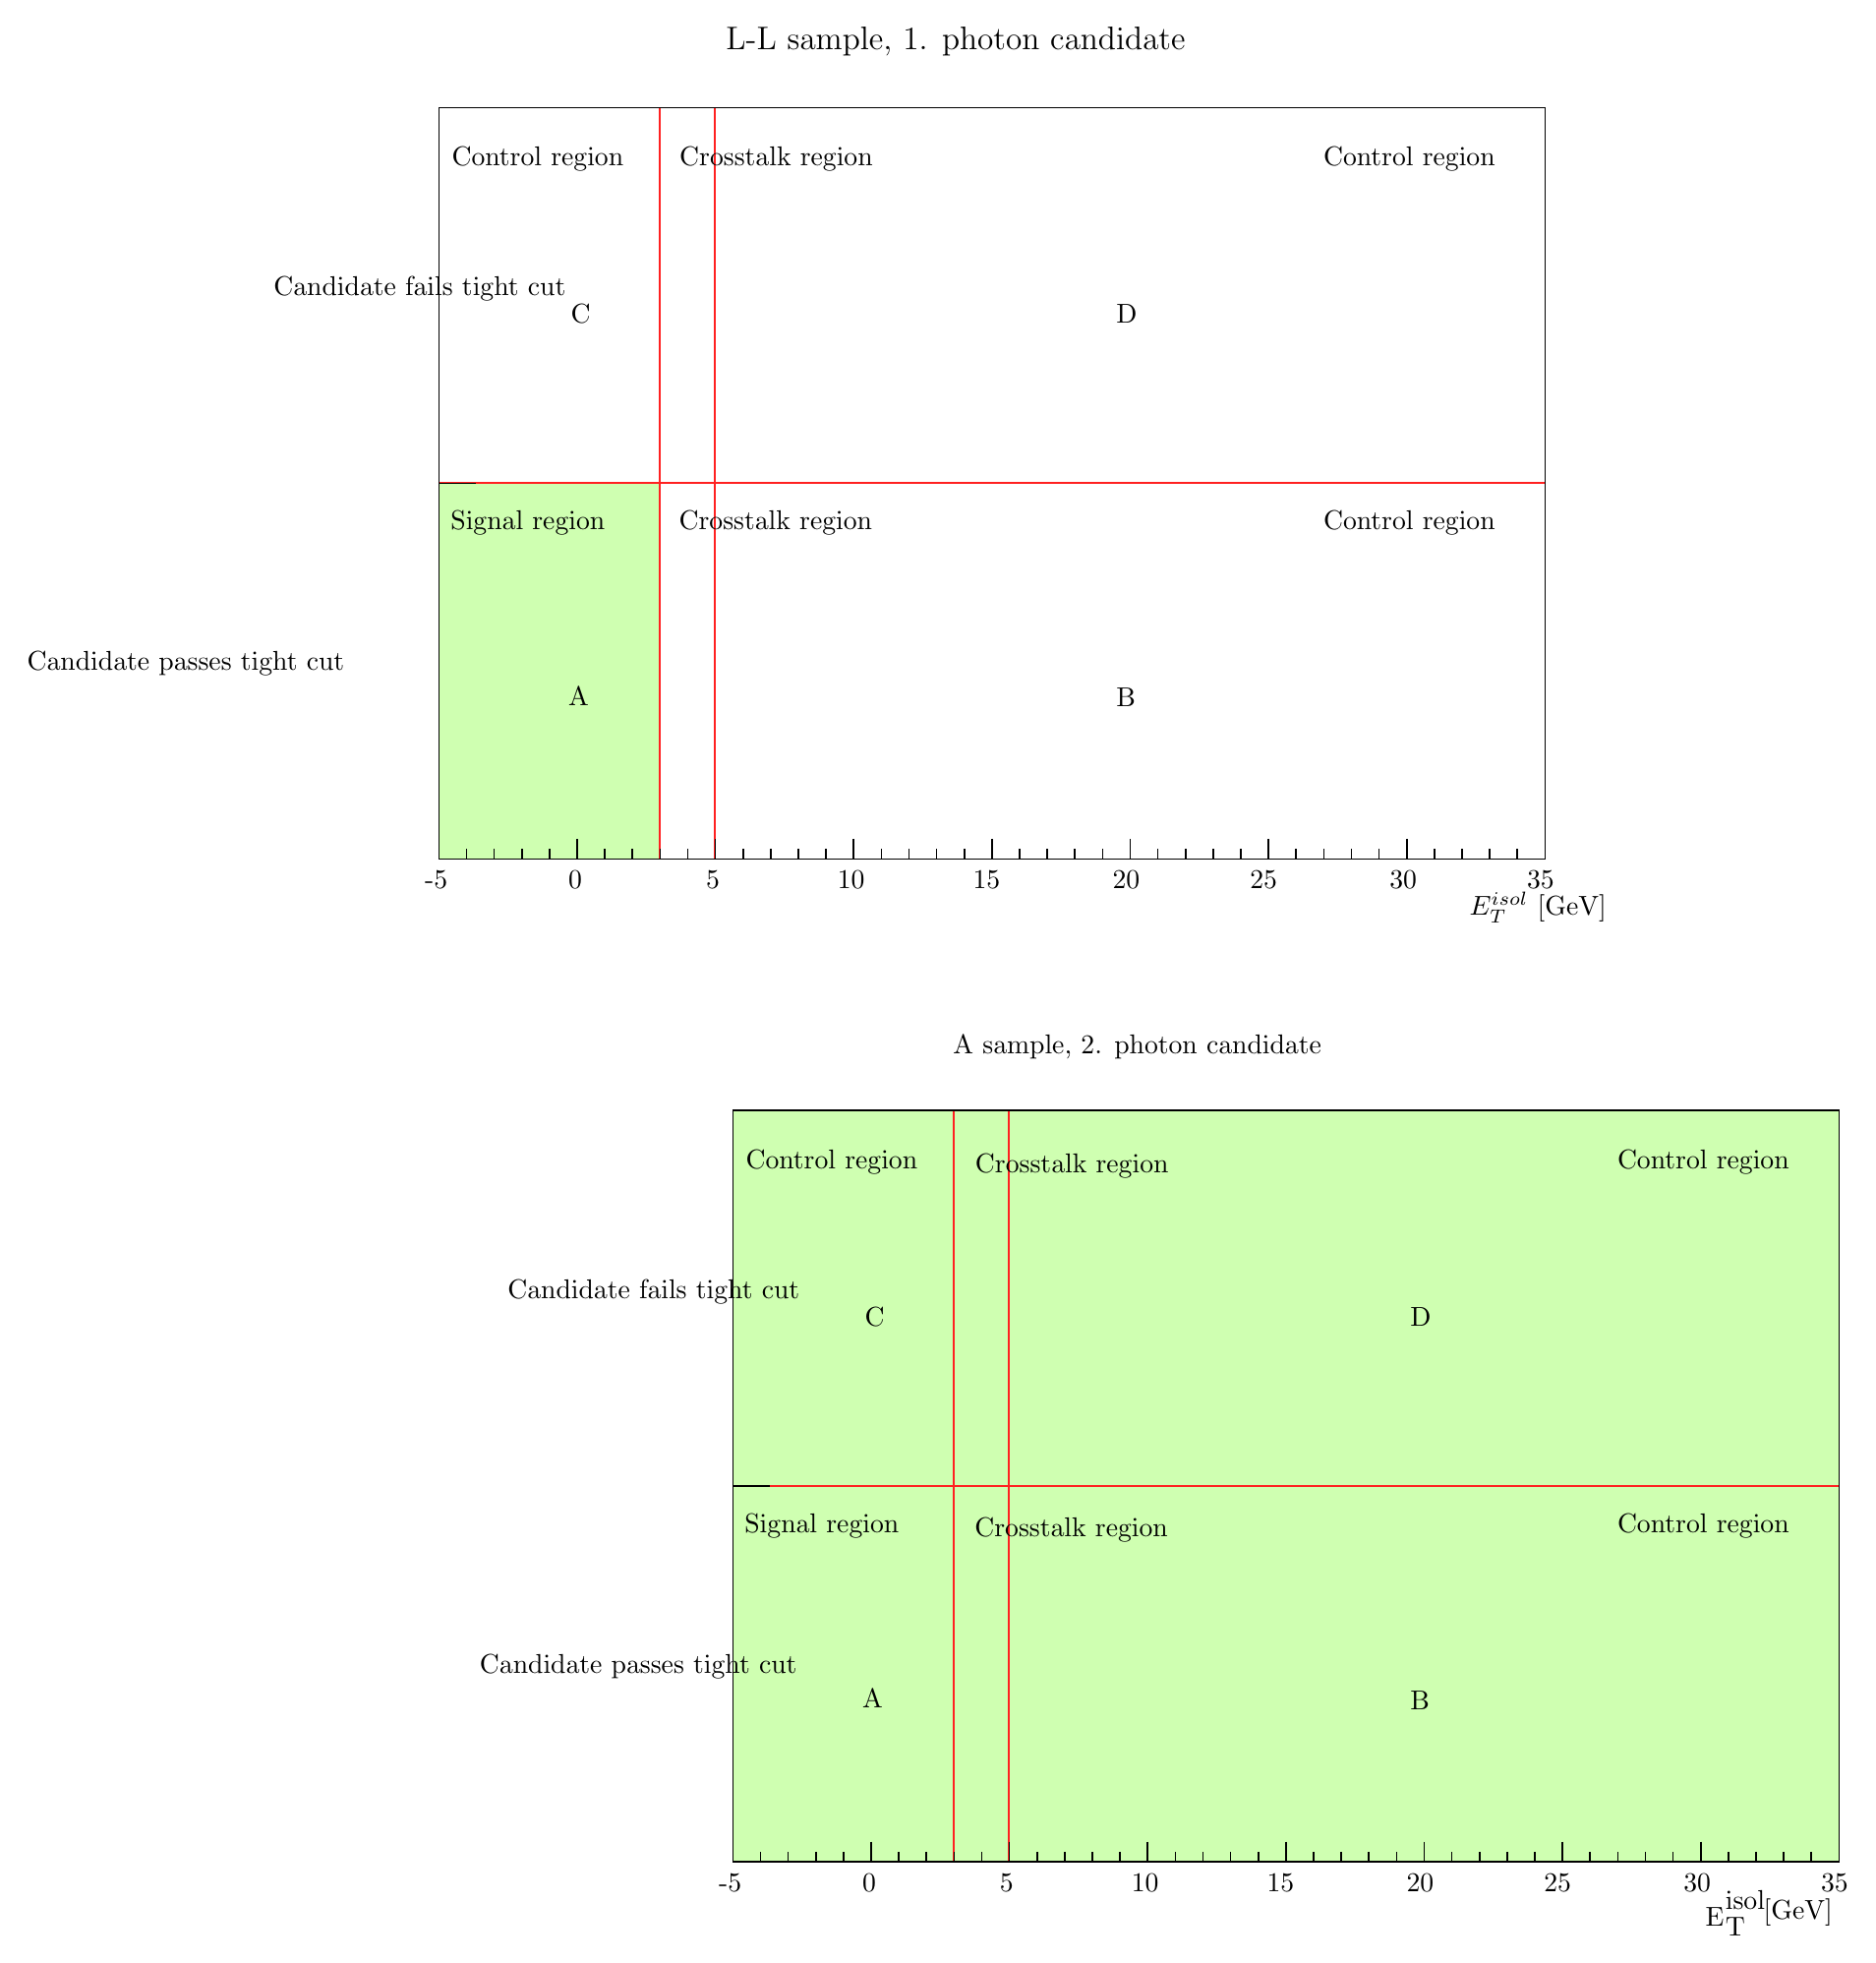
\begin{tikzpicture}[y=0.80pt,x=0.80pt,yscale=-1, inner sep=0pt, outer sep=0pt]
\begin{scope}[cm={{1.25,0.0,0.0,-1.25,(-13.27413,426.52708)}}]
  \path (183.7010,35.0756) -- (184.8410,173.3622) .. controls (293.0398,-30.3271)
    and (463.8486,-48.9835) .. (617.6873,-56.4777) -- (211.0481,-57.0722);
  \path (211.0481,-57.0722) -- (211.0481,-333.5155) .. controls
    (200.9477,-326.3547) and (154.0391,-196.6526) .. (102.9025,34.7274) ..
    controls (108.0367,36.5109) and (183.7010,35.0756) .. (183.7010,35.0756);
  \path[xscale=1.000,yscale=-1.000,fill=ccfffb1,rounded corners=0.0000cm]
    (103.2024,-173.6154) rectangle (184.1248,-35.3116);
      \path[cm={{1.0,0.0,0.0,-1.0,(482.08739,11.7195)}}] (0,0) node[above right]
        (text32) {$E_T^{isol}$ [GeV]};
      %% \path[cm={{1.0,0.0,0.0,-1.0,(468.046,17.5792)}}] (0,0) node[above right]
      %%   (text44) {isol};
      %% \path[cm={{1.0,0.0,0.0,-1.0,(468.046,8.05713)}}] (0,0) node[above right]
      %%   (text56) {T};
      %% \path[cm={{1.0,0.0,0.0,-1.0,(460.721,11.7195)}}] (0,0) node[above right]
      %%   (text68) {E};
      \path[cm={{1.0,0.0,0.0,-1.0,(10.2545,102.545)}}] (0,0) node[above]
        (text272) {Candidate passes tight cut};
      \path[cm={{1.0,0.0,0.0,-1.0,(20.5091,240.249)}}] (75.712936,0) node[above]
        (text284) {Candidate fails tight cut};
  \path[xscale=1.000,yscale=-1.000,fill=black] (293.1788,-330.14844) node[above
  ] (text3287) {\large L-L sample, 1. photon candidate};
  \path[draw=cff2121,fill=black,line width=0.640pt] (103.6535,173.3843) --
    (509.4882,173.3843);
  \path[draw=cff2121,fill=black,line join=round,line cap=butt,miter
    limit=4.00,line width=0.959pt] (184.4006,35.3548) -- (184.4006,311.3786);
  \path[draw=cff2121,fill=black,line join=round,line cap=butt,miter
    limit=4.00,line width=0.958pt] (204.6827,35.0066) -- (204.6827,311.1006);
  \path[draw=black,line join=miter,line cap=butt,miter limit=10.00,line
    width=0.600pt] (103.2780,35.1584) -- (509.7970,35.1584) -- (509.7970,311.2984)
    -- (103.2780,311.2984) -- (103.2780,35.1584) -- cycle;
  \path[draw=black,line join=miter,line cap=butt,miter limit=10.00,line
    width=0.600pt] (103.2780,35.1584) -- (509.7970,35.1584) -- (509.7970,311.2984)
    -- (103.2780,311.2984) -- (103.2780,35.1584) -- cycle;
  \path[draw=black,line join=miter,line cap=butt,miter limit=10.00,line
    width=0.600pt] (103.2780,35.1584) -- (509.7970,35.1584);
  \path[draw=black,line join=miter,line cap=butt,miter limit=10.00,line
    width=0.600pt] (103.2780,42.5955) -- (103.2780,35.1584);
  \path[draw=black,line join=miter,line cap=butt,miter limit=10.00,line
    width=0.600pt] (113.4410,38.8769) -- (113.4410,35.1584);
  \path[draw=black,line join=miter,line cap=butt,miter limit=10.00,line
    width=0.600pt] (123.6040,38.8769) -- (123.6040,35.1584);
  \path[draw=black,line join=miter,line cap=butt,miter limit=10.00,line
    width=0.600pt] (133.7670,38.8769) -- (133.7670,35.1584);
  \path[draw=black,line join=miter,line cap=butt,miter limit=10.00,line
    width=0.600pt] (143.9300,38.8769) -- (143.9300,35.1584);
  \path[draw=black,line join=miter,line cap=butt,miter limit=10.00,line
    width=0.600pt] (154.0930,42.5955) -- (154.0930,35.1584);
  \path[draw=black,line join=miter,line cap=butt,miter limit=10.00,line
    width=0.600pt] (164.2560,38.8769) -- (164.2560,35.1584);
  \path[draw=black,line join=miter,line cap=butt,miter limit=10.00,line
    width=0.600pt] (174.4190,38.8769) -- (174.4190,35.1584);
  \path[draw=black,line join=miter,line cap=butt,miter limit=10.00,line
    width=0.600pt] (184.5820,38.8769) -- (184.5820,35.1584);
  \path[draw=black,line join=miter,line cap=butt,miter limit=10.00,line
    width=0.600pt] (194.7450,38.8769) -- (194.7450,35.1584);
  \path[draw=black,line join=miter,line cap=butt,miter limit=10.00,line
    width=0.600pt] (204.9080,42.5955) -- (204.9080,35.1584);
  \path[draw=black,line join=miter,line cap=butt,miter limit=10.00,line
    width=0.600pt] (215.0700,38.8769) -- (215.0700,35.1584);
  \path[draw=black,line join=miter,line cap=butt,miter limit=10.00,line
    width=0.600pt] (225.2330,38.8769) -- (225.2330,35.1584);
  \path[draw=black,line join=miter,line cap=butt,miter limit=10.00,line
    width=0.600pt] (235.3960,38.8769) -- (235.3960,35.1584);
  \path[draw=black,line join=miter,line cap=butt,miter limit=10.00,line
    width=0.600pt] (245.5590,38.8769) -- (245.5590,35.1584);
  \path[draw=black,line join=miter,line cap=butt,miter limit=10.00,line
    width=0.600pt] (255.7220,42.5955) -- (255.7220,35.1584);
  \path[draw=black,line join=miter,line cap=butt,miter limit=10.00,line
    width=0.600pt] (265.8850,38.8769) -- (265.8850,35.1584);
  \path[draw=black,line join=miter,line cap=butt,miter limit=10.00,line
    width=0.600pt] (276.0480,38.8769) -- (276.0480,35.1584);
  \path[draw=black,line join=miter,line cap=butt,miter limit=10.00,line
    width=0.600pt] (286.2110,38.8769) -- (286.2110,35.1584);
  \path[draw=black,line join=miter,line cap=butt,miter limit=10.00,line
    width=0.600pt] (296.3740,38.8769) -- (296.3740,35.1584);
  \path[draw=black,line join=miter,line cap=butt,miter limit=10.00,line
    width=0.600pt] (306.5370,42.5955) -- (306.5370,35.1584);
  \path[draw=black,line join=miter,line cap=butt,miter limit=10.00,line
    width=0.600pt] (316.7000,38.8769) -- (316.7000,35.1584);
  \path[draw=black,line join=miter,line cap=butt,miter limit=10.00,line
    width=0.600pt] (326.8630,38.8769) -- (326.8630,35.1584);
  \path[draw=black,line join=miter,line cap=butt,miter limit=10.00,line
    width=0.600pt] (337.0260,38.8769) -- (337.0260,35.1584);
  \path[draw=black,line join=miter,line cap=butt,miter limit=10.00,line
    width=0.600pt] (347.1890,38.8769) -- (347.1890,35.1584);
  \path[draw=black,line join=miter,line cap=butt,miter limit=10.00,line
    width=0.600pt] (357.3520,42.5955) -- (357.3520,35.1584);
  \path[draw=black,line join=miter,line cap=butt,miter limit=10.00,line
    width=0.600pt] (367.5150,38.8769) -- (367.5150,35.1584);
  \path[draw=black,line join=miter,line cap=butt,miter limit=10.00,line
    width=0.600pt] (377.6780,38.8769) -- (377.6780,35.1584);
  \path[draw=black,line join=miter,line cap=butt,miter limit=10.00,line
    width=0.600pt] (387.8410,38.8769) -- (387.8410,35.1584);
  \path[draw=black,line join=miter,line cap=butt,miter limit=10.00,line
    width=0.600pt] (398.0040,38.8769) -- (398.0040,35.1584);
  \path[draw=black,line join=miter,line cap=butt,miter limit=10.00,line
    width=0.600pt] (408.1670,42.5955) -- (408.1670,35.1584);
  \path[draw=black,line join=miter,line cap=butt,miter limit=10.00,line
    width=0.600pt] (418.3300,38.8769) -- (418.3300,35.1584);
  \path[draw=black,line join=miter,line cap=butt,miter limit=10.00,line
    width=0.600pt] (428.4930,38.8769) -- (428.4930,35.1584);
  \path[draw=black,line join=miter,line cap=butt,miter limit=10.00,line
    width=0.600pt] (438.6560,38.8769) -- (438.6560,35.1584);
  \path[draw=black,line join=miter,line cap=butt,miter limit=10.00,line
    width=0.600pt] (448.8190,38.8769) -- (448.8190,35.1584);
  \path[draw=black,line join=miter,line cap=butt,miter limit=10.00,line
    width=0.600pt] (458.9820,42.5955) -- (458.9820,35.1584);
  \path[draw=black,line join=miter,line cap=butt,miter limit=10.00,line
    width=0.600pt] (469.1450,38.8769) -- (469.1450,35.1584);
  \path[draw=black,line join=miter,line cap=butt,miter limit=10.00,line
    width=0.600pt] (479.3080,38.8769) -- (479.3080,35.1584);
  \path[draw=black,line join=miter,line cap=butt,miter limit=10.00,line
    width=0.600pt] (489.4710,38.8769) -- (489.4710,35.1584);
  \path[draw=black,line join=miter,line cap=butt,miter limit=10.00,line
    width=0.600pt] (499.6340,38.8769) -- (499.6340,35.1584);
  \path[draw=black,line join=miter,line cap=butt,miter limit=10.00,line
    width=0.600pt] (509.7970,42.5955) -- (509.7970,35.1584);
      \path[cm={{1.0,0.0,0.0,-1.0,(98.1505,24.1714)}}] (0,0) node[above right]
        (text162) {-5};
      \path[cm={{1.0,0.0,0.0,-1.0,(150.888,24.1714)}}] (0,0) node[above right]
        (text174) {0};
      \path[cm={{1.0,0.0,0.0,-1.0,(201.428,24.1714)}}] (0,0) node[above right]
        (text186) {5};
      \path[cm={{1.0,0.0,0.0,-1.0,(249.771,24.1714)}}] (0,0) node[above right]
        (text198) {10};
      \path[cm={{1.0,0.0,0.0,-1.0,(299.579,24.1714)}}] (0,0) node[above right]
        (text210) {15};
      \path[cm={{1.0,0.0,0.0,-1.0,(350.852,24.1714)}}] (0,0) node[above right]
        (text222) {20};
      \path[cm={{1.0,0.0,0.0,-1.0,(401.392,24.1714)}}] (0,0) node[above right]
        (text234) {25};
      \path[cm={{1.0,0.0,0.0,-1.0,(452.664,24.1714)}}] (0,0) node[above right]
        (text246) {30};
      \path[cm={{1.0,0.0,0.0,-1.0,(503.205,24.1714)}}] (0,0) node[above right]
        (text258) {35};
  \path[draw=black,line join=miter,line cap=butt,miter limit=10.00,line
    width=0.600pt] (103.2780,35.1584) -- (103.2780,311.2980);
  \path[draw=black,line join=miter,line cap=butt,miter limit=10.00,line
    width=0.600pt] (116.8620,35.1584) -- (103.2780,35.1584);
  \path[draw=black,line join=miter,line cap=butt,miter limit=10.00,line
    width=0.600pt] (116.8620,173.2280) -- (103.2780,173.2280);
  \path[xscale=1.000,yscale=-1.000,fill=black] (150.91505,-91.642014) node[above
    right] (text4067) {A};
  \path[xscale=1.000,yscale=-1.000,fill=black] (352.27527,-91.221642) node[above
    right] (text4071) {B};
  \path[xscale=1.000,yscale=-1.000,fill=black] (352.27527,-232.04767) node[above
    right] (text4075) {D};
  \path[xscale=1.000,yscale=-1.000,fill=black] (151.7558,-232.04765) node[above
    right] (text4079) {C};
  \path[xscale=1.000,yscale=-1.000,fill=black] (107.61631,-154.27806) node[above
    right] (text4093) {Signal region};
  \path[xscale=1.000,yscale=-1.000,fill=black] (428.36334,-154.27806) node[above
    right] (text4093-2) {Control region};
  \path[xscale=1.000,yscale=-1.000,fill=black] (108.03668,-287.9577) node[above
    right] (text4093-2-7) {Control region};
  \path[xscale=1.000,yscale=-1.000,fill=black] (428.36334,-287.9577) node[above
    right] (text4093-2-5) {Control region};
  \path[xscale=1.000,yscale=-1.000,fill=ccfffb1,rounded corners=0.0000cm]
    (211.2390,57.5017) rectangle (617.6511,333.1354);
  \begin{scope}[shift={(108.03668,-368.44696)}]
      \path[cm={{1.0,0.0,0.0,-1.0,(482.08739,11.7195)}}] (0,0) node[above right]
        (text32-3) {[GeV]};
  \end{scope}
  \begin{scope}[shift={(108.03668,-368.44696)}]
      \path[cm={{1.0,0.0,0.0,-1.0,(468.046,17.5792)}}] (0,0) node[above right]
        (text44-7) {isol};
  \end{scope}
  \begin{scope}[shift={(108.03668,-368.44696)}]
      \path[cm={{1.0,0.0,0.0,-1.0,(468.046,8.05713)}}] (0,0) node[above right]
        (text56-8) {T};
  \end{scope}
  \begin{scope}[shift={(108.03668,-368.44696)}]
      \path[cm={{1.0,0.0,0.0,-1.0,(460.721,11.7195)}}] (0,0) node[above right]
        (text68-5) {E};
  \end{scope}
  \begin{scope}[shift={(108.03668,-368.44696)}]
      \path[cm={{1.0,0.0,0.0,-1.0,(10.2545,102.545)}}] (0,0) node[above right]
        (text272-4) {Candidate passes tight cut};
  \end{scope}
  \begin{scope}[shift={(108.03668,-368.44696)}]
      \path[cm={{1.0,0.0,0.0,-1.0,(20.5091,240.249)}}] (0,0) node[above right]
        (text284-4) {Candidate fails tight cut};
  \end{scope}
  \path[xscale=1.000,yscale=-1.000,fill=black] (292.25851,38.298531) node[above
    right] (text3287-5) {A sample, 2. photon candidate};
  \path[draw=cff2121,fill=black,line width=0.640pt] (211.6902,-195.0626) --
    (617.5249,-195.0626);
  \path[draw=cff2121,fill=black,line join=round,line cap=butt,miter
    limit=4.00,line width=0.959pt] (292.4373,-333.0921) -- (292.4373,-57.0683);
  \path[draw=cff2121,fill=black,line join=round,line cap=butt,miter
    limit=4.00,line width=0.958pt] (312.7194,-333.4404) -- (312.7194,-57.3464);
  \path[draw=black,line join=miter,line cap=butt,miter limit=10.00,line
    width=0.600pt] (211.3147,-333.2886) -- (617.8337,-333.2886) --
    (617.8337,-57.1486) -- (211.3147,-57.1486) -- (211.3147,-333.2886) -- cycle;
  \path[draw=black,line join=miter,line cap=butt,miter limit=10.00,line
    width=0.600pt] (211.3147,-333.2886) -- (617.8337,-333.2886) --
    (617.8337,-57.1486) -- (211.3147,-57.1486) -- (211.3147,-333.2886) -- cycle;
  \path[draw=black,line join=miter,line cap=butt,miter limit=10.00,line
    width=0.600pt] (211.3147,-333.2886) -- (617.8337,-333.2886);
  \path[draw=black,line join=miter,line cap=butt,miter limit=10.00,line
    width=0.600pt] (211.3147,-325.8515) -- (211.3147,-333.2886);
  \path[draw=black,line join=miter,line cap=butt,miter limit=10.00,line
    width=0.600pt] (221.4777,-329.5701) -- (221.4777,-333.2886);
  \path[draw=black,line join=miter,line cap=butt,miter limit=10.00,line
    width=0.600pt] (231.6407,-329.5701) -- (231.6407,-333.2886);
  \path[draw=black,line join=miter,line cap=butt,miter limit=10.00,line
    width=0.600pt] (241.8037,-329.5701) -- (241.8037,-333.2886);
  \path[draw=black,line join=miter,line cap=butt,miter limit=10.00,line
    width=0.600pt] (251.9667,-329.5701) -- (251.9667,-333.2886);
  \path[draw=black,line join=miter,line cap=butt,miter limit=10.00,line
    width=0.600pt] (262.1297,-325.8515) -- (262.1297,-333.2886);
  \path[draw=black,line join=miter,line cap=butt,miter limit=10.00,line
    width=0.600pt] (272.2927,-329.5701) -- (272.2927,-333.2886);
  \path[draw=black,line join=miter,line cap=butt,miter limit=10.00,line
    width=0.600pt] (282.4557,-329.5701) -- (282.4557,-333.2886);
  \path[draw=black,line join=miter,line cap=butt,miter limit=10.00,line
    width=0.600pt] (292.6187,-329.5701) -- (292.6187,-333.2886);
  \path[draw=black,line join=miter,line cap=butt,miter limit=10.00,line
    width=0.600pt] (302.7817,-329.5701) -- (302.7817,-333.2886);
  \path[draw=black,line join=miter,line cap=butt,miter limit=10.00,line
    width=0.600pt] (312.9447,-325.8515) -- (312.9447,-333.2886);
  \path[draw=black,line join=miter,line cap=butt,miter limit=10.00,line
    width=0.600pt] (323.1067,-329.5701) -- (323.1067,-333.2886);
  \path[draw=black,line join=miter,line cap=butt,miter limit=10.00,line
    width=0.600pt] (333.2697,-329.5701) -- (333.2697,-333.2886);
  \path[draw=black,line join=miter,line cap=butt,miter limit=10.00,line
    width=0.600pt] (343.4327,-329.5701) -- (343.4327,-333.2886);
  \path[draw=black,line join=miter,line cap=butt,miter limit=10.00,line
    width=0.600pt] (353.5957,-329.5701) -- (353.5957,-333.2886);
  \path[draw=black,line join=miter,line cap=butt,miter limit=10.00,line
    width=0.600pt] (363.7587,-325.8515) -- (363.7587,-333.2886);
  \path[draw=black,line join=miter,line cap=butt,miter limit=10.00,line
    width=0.600pt] (373.9217,-329.5701) -- (373.9217,-333.2886);
  \path[draw=black,line join=miter,line cap=butt,miter limit=10.00,line
    width=0.600pt] (384.0847,-329.5701) -- (384.0847,-333.2886);
  \path[draw=black,line join=miter,line cap=butt,miter limit=10.00,line
    width=0.600pt] (394.2477,-329.5701) -- (394.2477,-333.2886);
  \path[draw=black,line join=miter,line cap=butt,miter limit=10.00,line
    width=0.600pt] (404.4107,-329.5701) -- (404.4107,-333.2886);
  \path[draw=black,line join=miter,line cap=butt,miter limit=10.00,line
    width=0.600pt] (414.5737,-325.8515) -- (414.5737,-333.2886);
  \path[draw=black,line join=miter,line cap=butt,miter limit=10.00,line
    width=0.600pt] (424.7367,-329.5701) -- (424.7367,-333.2886);
  \path[draw=black,line join=miter,line cap=butt,miter limit=10.00,line
    width=0.600pt] (434.8997,-329.5701) -- (434.8997,-333.2886);
  \path[draw=black,line join=miter,line cap=butt,miter limit=10.00,line
    width=0.600pt] (445.0627,-329.5701) -- (445.0627,-333.2886);
  \path[draw=black,line join=miter,line cap=butt,miter limit=10.00,line
    width=0.600pt] (455.2257,-329.5701) -- (455.2257,-333.2886);
  \path[draw=black,line join=miter,line cap=butt,miter limit=10.00,line
    width=0.600pt] (465.3887,-325.8515) -- (465.3887,-333.2886);
  \path[draw=black,line join=miter,line cap=butt,miter limit=10.00,line
    width=0.600pt] (475.5517,-329.5701) -- (475.5517,-333.2886);
  \path[draw=black,line join=miter,line cap=butt,miter limit=10.00,line
    width=0.600pt] (485.7147,-329.5701) -- (485.7147,-333.2886);
  \path[draw=black,line join=miter,line cap=butt,miter limit=10.00,line
    width=0.600pt] (495.8777,-329.5701) -- (495.8777,-333.2886);
  \path[draw=black,line join=miter,line cap=butt,miter limit=10.00,line
    width=0.600pt] (506.0407,-329.5701) -- (506.0407,-333.2886);
  \path[draw=black,line join=miter,line cap=butt,miter limit=10.00,line
    width=0.600pt] (516.2037,-325.8515) -- (516.2037,-333.2886);
  \path[draw=black,line join=miter,line cap=butt,miter limit=10.00,line
    width=0.600pt] (526.3667,-329.5701) -- (526.3667,-333.2886);
  \path[draw=black,line join=miter,line cap=butt,miter limit=10.00,line
    width=0.600pt] (536.5297,-329.5701) -- (536.5297,-333.2886);
  \path[draw=black,line join=miter,line cap=butt,miter limit=10.00,line
    width=0.600pt] (546.6927,-329.5701) -- (546.6927,-333.2886);
  \path[draw=black,line join=miter,line cap=butt,miter limit=10.00,line
    width=0.600pt] (556.8557,-329.5701) -- (556.8557,-333.2886);
  \path[draw=black,line join=miter,line cap=butt,miter limit=10.00,line
    width=0.600pt] (567.0187,-325.8515) -- (567.0187,-333.2886);
  \path[draw=black,line join=miter,line cap=butt,miter limit=10.00,line
    width=0.600pt] (577.1817,-329.5701) -- (577.1817,-333.2886);
  \path[draw=black,line join=miter,line cap=butt,miter limit=10.00,line
    width=0.600pt] (587.3447,-329.5701) -- (587.3447,-333.2886);
  \path[draw=black,line join=miter,line cap=butt,miter limit=10.00,line
    width=0.600pt] (597.5077,-329.5701) -- (597.5077,-333.2886);
  \path[draw=black,line join=miter,line cap=butt,miter limit=10.00,line
    width=0.600pt] (607.6707,-329.5701) -- (607.6707,-333.2886);
  \path[draw=black,line join=miter,line cap=butt,miter limit=10.00,line
    width=0.600pt] (617.8337,-325.8515) -- (617.8337,-333.2886);
  \begin{scope}[shift={(108.03668,-368.44696)}]
      \path[cm={{1.0,0.0,0.0,-1.0,(98.1505,24.1714)}}] (0,0) node[above right]
        (text162-3) {-5};
  \end{scope}
  \begin{scope}[shift={(108.03668,-368.44696)}]
      \path[cm={{1.0,0.0,0.0,-1.0,(150.888,24.1714)}}] (0,0) node[above right]
        (text174-6) {0};
  \end{scope}
  \begin{scope}[shift={(108.03668,-368.44696)}]
      \path[cm={{1.0,0.0,0.0,-1.0,(201.428,24.1714)}}] (0,0) node[above right]
        (text186-9) {5};
  \end{scope}
  \begin{scope}[shift={(108.03668,-368.44696)}]
      \path[cm={{1.0,0.0,0.0,-1.0,(249.771,24.1714)}}] (0,0) node[above right]
        (text198-9) {10};
  \end{scope}
  \begin{scope}[shift={(108.03668,-368.44696)}]
      \path[cm={{1.0,0.0,0.0,-1.0,(299.579,24.1714)}}] (0,0) node[above right]
        (text210-5) {15};
  \end{scope}
  \begin{scope}[shift={(108.03668,-368.44696)}]
      \path[cm={{1.0,0.0,0.0,-1.0,(350.852,24.1714)}}] (0,0) node[above right]
        (text222-1) {20};
  \end{scope}
  \begin{scope}[shift={(108.03668,-368.44696)}]
      \path[cm={{1.0,0.0,0.0,-1.0,(401.392,24.1714)}}] (0,0) node[above right]
        (text234-0) {25};
  \end{scope}
  \begin{scope}[shift={(108.03668,-368.44696)}]
      \path[cm={{1.0,0.0,0.0,-1.0,(452.664,24.1714)}}] (0,0) node[above right]
        (text246-6) {30};
  \end{scope}
  \begin{scope}[shift={(108.03668,-368.44696)}]
      \path[cm={{1.0,0.0,0.0,-1.0,(503.205,24.1714)}}] (0,0) node[above right]
        (text258-7) {35};
  \end{scope}
  \path[draw=black,line join=miter,line cap=butt,miter limit=10.00,line
    width=0.600pt] (211.3147,-333.2886) -- (211.3147,-57.1490);
  \path[draw=black,line join=miter,line cap=butt,miter limit=10.00,line
    width=0.600pt] (224.8987,-333.2886) -- (211.3147,-333.2886);
  \path[draw=black,line join=miter,line cap=butt,miter limit=10.00,line
    width=0.600pt] (224.8987,-195.2190) -- (211.3147,-195.2190);
  \path[xscale=1.000,yscale=-1.000,fill=black] (258.95172,276.80496) node[above
    right] (text4067-3) {A};
  \path[xscale=1.000,yscale=-1.000,fill=black] (460.31192,277.22531) node[above
    right] (text4071-1) {B};
  \path[xscale=1.000,yscale=-1.000,fill=black] (460.31192,136.39929) node[above
    right] (text4075-2) {D};
  \path[xscale=1.000,yscale=-1.000,fill=black] (259.79248,136.39931) node[above
    right] (text4079-7) {C};
  \path[xscale=1.000,yscale=-1.000,fill=black] (215.65298,214.16888) node[above
    right] (text4093-6) {Signal region};
  \path[xscale=1.000,yscale=-1.000,fill=black] (536.40002,214.16888) node[above
    right] (text4093-2-1) {Control region};
  \path[xscale=1.000,yscale=-1.000,fill=black] (216.07336,80.489265) node[above
    right] (text4093-2-7-8) {Control region};
  \path[xscale=1.000,yscale=-1.000,fill=black] (536.40002,80.489265) node[above
    right] (text4093-2-5-1) {Control region};
  \path[cm={{0.0,-1.0,-1.0,0.0,(0.0,0.0)}},fill=black] (-287.9577,-191.74933)
    node[above right] (text4899) {Crosstalk region};
  \path[cm={{0.0,-1.0,-1.0,0.0,(0.0,0.0)}},fill=black] (-154.27806,-191.53021)
    node[above right] (text4899-9) {Crosstalk region};
  \path[cm={{0.0,-1.0,-1.0,0.0,(0.0,0.0)}},fill=black] (82.160568,-300.43359)
    node[above right] (text4899-7) {Crosstalk region};
  \path[cm={{0.0,-1.0,-1.0,0.0,(0.0,0.0)}},fill=black] (215.84023,-300.21448)
    node[above right] (text4899-9-9) {Crosstalk region};
\end{scope}

\end{tikzpicture}
\end{infilsf}
